\section{Payload-Conditioned Trajectory Denoising}

In this section, we present our payload-conditioned diffusion model to generate pick-and-place trajectories that transport super-nominal payloads while obeying kinematic and dynamic constraints.

\subsection{Training Data}

Our payload-conditioned diffusion model (\Cref{sec:model}) is trained on $25,000$ time-parameterized, collision-free joint space trajectories (state dimension = DoF$\times3$, corresponding to joint angles, velocities, and accelerations) for tabletop pick-and-place motions. These trajectories are generated using a plan-and-filter pipeline that uses cuRobo, a GPU-accelerated trajectory optimization framework \cite{sundaralingam2023curobo}, followed by a dynamics validation step (\Cref{fig:data-generation}).
\begin{wrapfigure}{r}{0.5\textwidth}   % l or r = left / right, width = ~½ line
  \vspace{-1.2\baselineskip}            % tighten top gap (optional)
  \centering
  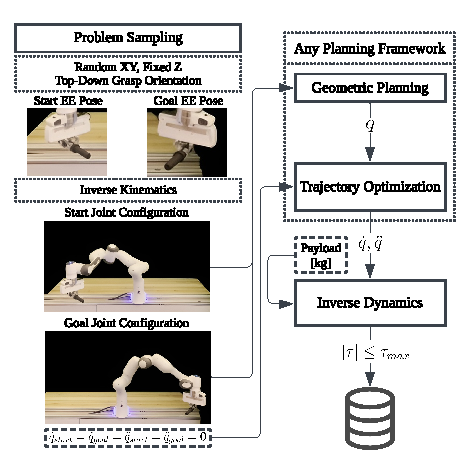
\includegraphics[width=\linewidth]{graphics/datagen.pdf}
  \caption{Plan-and-filter process to create training data.}
  \label{fig:data-generation}
  \vspace{-1.4\baselineskip}            % tighten bottom gap (optional)
\end{wrapfigure}
First, trajectories are generated for the 7DoF Franka Emika Panda robot arm with an effective payload mass of $0$kg.
Second, to ensure that payload-induced joint torques remain within hardware limits, each trajectory is verified through an analytically-derived dynamics model parameterized on real-world data \cite{gaz2019dynamic}.
This model captures both the standard dynamic elements (inertia, Coriolis, and gravity) and velocity-dependent joint friction.
By using a dynamics model fitted to real robot trajectory data, we ensure that our training dataset reflects the physical constraints observed in hardware.

This dynamics verification step utilizes a complete robot model where $q$, $\dot{q}$, $\ddot{q}$, and $\tau$ are $7\times1$ vectors representing joint angles, velocities, accelerations, and torques respectively.
The dynamics matrices include: $M(q)$ ($7\times7$ positive-definite, symmetric joint inertia matrix), $C(q,\dot{q})$ ($7\times7$ Coriolis/centrifugal matrix), $g(q)$ ($7\times1$ gravity compensation torque vector), and $f(\dot{q})$ ($7\times1$ joint friction torque vector). External task space forces $F_{ext}$ ($6\times1$) map to joint torques through the Jacobian $J(q)$ ($7\times7$).
The dynamics model is parameterized as:
\begin{equation}\label{eq:arm-dyns}
    \tau = M(q)\ddot{q} + C(q, \dot{q})\dot{q} + g(q) + f(\dot{q}) + J^{-1}(q)F_{ext}
\end{equation}
Note that this analytically-derived model represents the robot without external payloads which can affect model accuracy when considering varying payload masses in real-world deployment.
To account for payload-induced joint torques, we model the gravitational effects as a 6D Cartesian wrench transformed from the world frame to the end-effector frame.
This frame transformation is critical for accurately projecting gravitational forces acting on the payload along the robot's embodiment.
We represent the external gravitational wrench $\bm{F}_g \in \mathbb{R}^6$ in the world frame with a simplified point mass model:
$\bm{F}_g = mg \cdot [0,\ 0,\ -1,\ 0,\ 0,\ 0]^T$
where $m \in \mathbb{R}^+$ denotes payload mass and $g \approx 9.81 \text{ m/s}^2$ is gravitational acceleration. This representation assumes force application at the object's center of mass, neglecting potential moment contributions.
The wrench's structure combines linear forces (first three components) and angular forces (last three components), which are
mapped to induced joint torques through the manipulator Jacobian, contributing to the total joint torque vector (\cref{eq:arm-dyns}).

The training dataset $\mathcal{D}$ is constructed from these trajectories that satisfy both kinematic and dynamic constraints. Each element $d_i \in \mathcal{D}$ is a tuple of trajectory $\bm{\pi}_i$ and maximum supported payload $m_i$. %, where $\bm{\pi}_i$ is as defined in \Cref{sec:diffusion}.
Each $m_i$ is the maximum supported payload mass for trajectory $i$ subject to $|\tau(\bm{\pi}_i, m_i)| \leq \tau_{max}$, $\forall t \in [0,T]$ where $\tau_t$ is computed via the dynamics equation (\cref{eq:arm-dyns}).
Having established our dataset $\mathcal{D}$ of dynamically feasible trajectories and their corresponding maximum payload limits, we now consider different ways of incorporating payload conditioning into the diffusion model architecture.

\vspace{-0.12in}

\subsection{Payload-Conditional Trajectory Generation}\label{sec:model}
\vspace{-0.1in}

We extend the diffusion policy architecture to condition trajectory generation on payload mass through global conditioning \cite{chi2023diffusionpolicy}. Unlike local conditioning where features influence each waypoint individually, global conditioning applies the mass embedding uniformly across the entire trajectory generation process, preserving dynamic feasibility across the generated motion (\Cref{fig:architecture}).
For each training trajectory $i$ with corresponding maximum supported payload mass $m_i \in \mathcal{D}$, we investigate four approaches to incorporate a target payload mass $p_i$ into an encoding vector $\mathcal{P}_i$.
The payload encoding $\mathcal{P}$ is concatenated with a diffusion timestep embedding to form a global conditioning vector, which is then integrated into $\epsilon_\theta$ through either additive or affine transform conditioning \cite{perez2018film}.% (\Cref{sec:misc-design}).
\begin{wrapfigure}{l}{0.48\textwidth}   % l or r = left / right, width = ~½ line
  \vspace{-1.6\baselineskip}            % tighten top gap (optional)
  \centering
  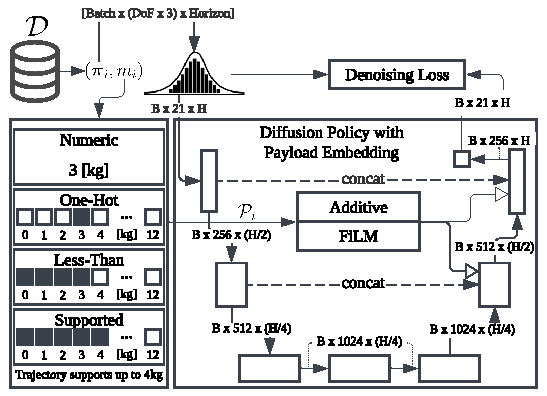
\includegraphics[width=\linewidth]{graphics/archnew.pdf}
  \caption{Our model conditions a 1D UNet denoising architecture \cite{chi2023diffusionpolicy} on various payload embeddings.}
  \label{fig:architecture}
  \vspace{-1.3\baselineskip}            % tighten bottom gap (optional)
\end{wrapfigure}
We consider the following approaches for designing $\mathcal{P}$.
\noindent\textbf{Numeric Input.} A random supported mass scalar $p_i \sim \mathcal{U}(0, m_i)$ is sampled and fed directly to the network. This approach naturally supports continuous payload values during inference, despite training on a discrete set of payload values.
\noindent\textbf{One-Hot Encoding.} For a system supporting payloads from $0-18$kg in $1$kg increments, a random supported mass $p_i \sim \mathcal{U}(0, m_i)$ is encoded as a $19$-dimensional binary vector with a single non-zero entry at index $\lceil p_i \rceil$.
While this categorical representation simplifies the learning task by discretizing the payload space, it constrains inference to the discrete payload values seen during training.
During inference, continuous payload masses must be quantized to their ceiling value $\lceil p \rceil$ before input to the denoising network, ensuring a tight upper bound for conservative operation.
\noindent\textbf{Less-Than Encoding.} This encoding exploits the logical constraint that trajectories supporting a given payload must also support all lighter payloads.
For a random supported mass $p_i \sim \mathcal{U}(0, m_i)$, we construct a $19$-dimensional binary vector where entries are $1$ for indices $j \leq \lceil p_i \rceil$ and $0$ otherwise.
This representation directly encodes the downward compatibility constraint into the input space, potentially improving the network's ability to learn and respect payload-dependent constraints.
During inference, continuous payload masses are similarly mapped to their ceiling value $\lceil p \rceil$ to construct the binary encoding.
\noindent\textbf{Supported-Range Encoding.}
This approach encodes the complete range of supported payloads for a given trajectory.
For training trajectory $i$ with maximum supported mass $m_i$, we construct a $19$-dimensional binary vector where entries are $1$ for indices $j \leq \lceil m_i \rceil$ and $0$ otherwise.
During training, this encoding preserves the full payload compatibility information from $\mathcal{D}$.
At inference time, for a target payload mass $p$, the encoding can be constructed either as a one-hot vector with a single non-zero entry at index $\lceil p \rceil$, or as a less-than encoding with ones for indices $j \leq \lceil p \rceil$.
This dual interpretation enables both trajectory generation for specific payloads and exploration of the learned manifold of payload-trajectory relationships.
Broadly, each encoding method presents trade-offs between generalization capability and training simplicity.